\newpage
\section{Slu\v cajevi upotrebe}
\subsection{Upravljanje nalozima}
\subsubsection{Registracija korisnika na sajtu restorana}
\begin{itemize}
    \item \textbf{Kratak opis}:
    Korisnik prvi put pristupa nalogu restorana i zato je neophodna registracija kako bi mogao poručiti hranu.
    \item \textbf{Učesnici}:
    Korisnik
    \item \textbf{Preduslovi}:
    Nema preduslova. 
    \item \textbf{Postuslovi}:
    Korisnik je registrovan. 
    \item \textbf{Glavni tok}:
    \begin{enumerate}
        \item Korisnik odlazi na nalog restorana i otvara formu za registraciju.
        \item Korisnik popunjava formu za registraciju.
        \item Sistem vrši validaciju registracije.
        \item Sistem beleži novog korisnika u bazi
        \item Sistem obaveštava korisnika o uspešnosti registracije.
    \end{enumerate}
\end{itemize}

\begin {itemize}
\item \textbf {Alternativni tokovi}: \\
 3.1. Korisnik nije uneo ispravne podatke za registraciju.\\
 Slučaj upotrebe se nastavlja na koraku 2 glavnog toka.
\end{itemize}
 \begin{itemize} 
    \item \textbf{Dodatne informacije}
    \begin{itemize}
        \item Neophodni podaci za registraciju korisnika su validna e-mail adresa, ime, prezime, adresa, korisničko ime i lozinka.
        \item Sistem validira novog korisnika tako što proverava da li već postoji nalog sa unetom e-mail adresom. Neophodno je i da korisničko ime bude jedinstveno.
    \end{itemize}
\end{itemize}
 
 
\subsubsection{Ocenjivanje usluge restorana}
\begin{itemize}
    \item \textbf{Kratak opis}:
    Korisniku je data mogućnost da napiše svoj utisak o usluzi restorana koji je vidljiv drugim korisnicima.
    \item \textbf{Učesnici}:
    Korisnik
    \item \textbf{Preduslovi}:
    Postojanje korisničkog naloga. 
    \item \textbf{Postuslovi}:
    Korisnik je napisao u komentaru svoj utisak
    o restoranu.
    \item \textbf{Glavni tok}:
   \begin{enumerate}
        \item Korisnik odlazi na nalog restorana i otvara stranicu Utisci.
        \item Korisnik popunjava formu za ostavljanje utiska.
        \item Sistem vrši validaciju utiska.
        \item Ažurira se stranica Utisci.
        \item Sistem obaveštava korisnika da je uspešno postavio komentar.
    \end{enumerate}
\end{itemize}
\begin{itemize}
\item \textbf {Alternativni tokovi}:\\ 
 3.1. Korisnik nije popunio sva obavezna polja.\\
 Slučaj upotrebe se nastavlja na koraku 2 glavnog toka.\\
 3.2. Korisnik je uneo e-mail adresu koja ne odgovara nijednom postojećem nalogu korisnika. \\
 Korisnik dobija odgovarajuću poruku i postavlja mu se pitanje da li želi da se registruje. \\
 Slučaj upotrebe se nastavlja na koraku 2 glavnog toka.
 
\quad 3.2.1. Korisnik potvrđuje da želi da se registruje.
Prelazi se na slučaj upotrebe ”3.1.1 Registracija korisnika na sajtu restorana".Nakon završetka tog slučaja upotrebe, slučaj upotrebe se vraća
na korak 2 glavnog toka. 

\quad 3.2.2. Korisnik ne želi da se registruje. Završava se slučaj upotrebe.
\end{itemize}

\begin{itemize} 
     \item \textbf{Dodatne informacije}
 \begin{itemize}
     \item Obavezna polja koja korisnik mora popuniti da bi ostavio utisak su validna e-mail adresa, ime i komentar.
    \item Sistem validira utisak tako što proverava da li postoji nalog korisnika kome odgovara uneta e-mail adresa.
 \end{itemize}
 \end{itemize}
 
 \subsubsection{Kreiranje naloga za radnika upravo zaposlenog u restoranu}
\begin{itemize}
    \item \textbf{Kratak opis}:
   Radniku koji je upravo zaposlen u restoranu potrebno je napraviti nalog kako bi imao pristup sistemu.
    \item \textbf{Učesnici}:
    Menadžer
    \item \textbf{Preduslovi}:
    Zaposleni je upravo dobio posao u restoranu.
    \item \textbf{Postuslovi}:
    Zaposleni ima svoj nalog. 
    \item \textbf{Glavni tok}:
   \begin{enumerate}
        \item Menadžer odlazi na veb stranicu i prijavljuje se unošenjem svog korisničkog imena i šifre.
        \item Menadžer otvara formu za unošenje novog naloga za zaposlene.
        \item Menadžer popunjava formu svim potrebnim podacima.
        \item Menadžer odredjuje prava pristupa nalozima zaposlenih.
        \item Menadžer potvrđuje unete podatke klikom na dugme 'Sačuvaj'.
        \item Sistem beleži novog zaposlenog u bazi.
        \item Sistem obaveštava zaposlenog o uspešnosti registracije slanjem e-mail poruke.
\end{enumerate}
\end{itemize}
\begin {itemize}
\item \textbf {Alternativni tokovi}:\\
 3.1. Menadžer nije uneo ispravne podatke za registraciju.\\
 Slučaj upotrebe se nastavlja na koraku 2 glavnog toka.
 \end{itemize}
 \begin{itemize} 
     \item \textbf{Dodatne informacije}
 \begin{itemize}
     \item Neophodni podaci za pravljenje naloga zaposlenom su validna e-mail adresa, ime, prezime, adresa, korisničko ime, lozinka, kao i odabir funkcije zaposlenog, čiji je nalog u nastanku.
    \item Sistem validira novog zaposlenog tako što proverava da li već postoji nalog sa unetom e-mail adresom. Neophodno je i da korisničko ime bude jedinstveno.
 \end{itemize}
 \end{itemize}

 \subsubsection{Deaktivacija naloga otpuštenog radnika}
 \begin{itemize}
    \item \textbf{Kratak opis}:
   Radniku koji je otpušten menadžer deaktivira nalog kako više ne bi imao pristup sistemu.
    \item \textbf{Učesnici}:
    Menadžer.
    \item \textbf{Preduslovi}:
    Radnik je dobio/dao otkaz u restoranu. Takođe, u sistemu postoji njegov nalog.
    \item \textbf{Postuslovi}:
    Radniku je deaktiviran nalog. 
    \item \textbf{Glavni tok}:
    \begin{enumerate}
        \item Menadžer odlazi na veb stranicu i prijavljuje se unošenjem svog korisničkog imena i šifre.
        \item Menadžer pronalazi nalog bivšeg zaposlenog.
        \item Menadžer deaktivira nalog klikom na dugme 'Deaktiviraj'.
        \item Menadžer potvrđuje unete promene klikom na dugme 'Sačuvaj'.
        \item Sistem beleži promene u bazi.
        \item Sistem obaveštava radnika o deaktivaciji naloga slanjem e-mail poruke.
    \end{enumerate}
\item \textbf{Dodatne informacije}
 \begin{itemize}
     \item Pri deaktivaciji naloga, nalog se ne briše, tako da u slučaju ponovnog zaposlenja, dovoljno je da menadžer aktivira postojeći nalog.
 \end{itemize}
 \end{itemize}
\newpage
\subsection{Upravljanje porudžbinom}
Na slici \ref{fig:slika3} je predstavljen dijagram stanja koji opisuje opšti tok upravljanja porudžbinom. U zavisnosti od toga da li među zalihama ima dovoljno namirnica, porudžbina se prihvata ili odbija.

\begin{figure}[ht]
    \leavevmode
    \begin{center}
    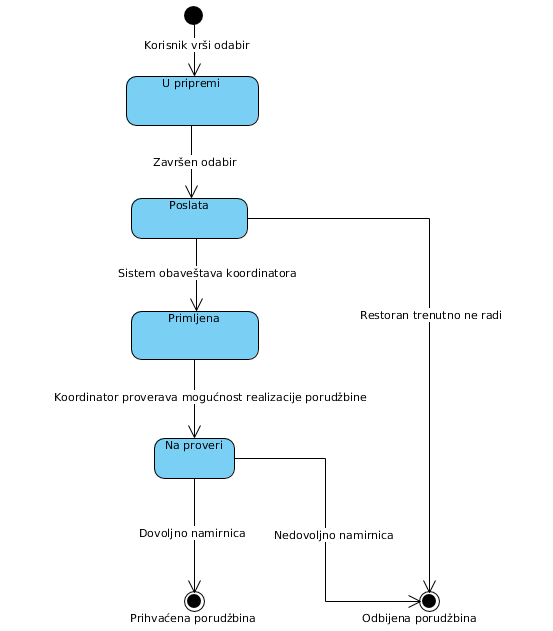
\includegraphics[height=0.6\textheight]{slike/Upravljanje_porudzbinom.png}
    \end{center}
    \caption{Dijagram stanja} % opis ce stajati ispod slike
    \label{fig:slika3}
\end{figure}


\subsubsection{Onlajn naručivanje}
\begin{itemize}
    \item \textbf{Kratak opis}: Korisnik naručuje željenu hranu putem veb stranice. Porudžbina biva prihvaćena ili odbijena od strane koordinatora.
    \item \textbf{Učesnici}: Korisnik, koordinator.
    \item \textbf{Preduslovi}: Postojanje korisničkog naloga.
    \item \textbf{Postuslovi}: Prihvaćena, odnosno odbijena porudžbina.
    \item \textbf{Glavni tok}:
    \begin{enumerate}
        \item Korisnik se prijavljuje na sajt restorana.
        \item Korisnik vrši odabir željenih proizvoda.
        \item Korisnik potvrđuje željenu porudžbinu klikom na dugme "Poruči".
        \item Sistem odbija porudžbinu u slučaju da restoran trenutno ne radi i obaveštava korisnika o tome.
        \item Sistem obaveštava koordinatora o prispeću zahteva.
        \item Koordinator proverava da li je moguće realizovati porudžbinu.
        \item Koordinator utvrđuje da svih namirnica potrebnih za datu porudžbinu ima u dovoljnim količinama.
        \item Koordinator beleži na cedulju detalje porudžbine.
        \item Koordinator prihvata porudžbinu klikom na dugme "Prihvati".
        \item Korisnik biva obavešten, od strane sistema, da je porudžbina prihvaćena ili ne.
     \end{enumerate}
     \item \textbf{Alternativni tokovi}:
     
     7.1. Koordinator utvrđuje da ne postoji dovoljna količina namirnica za pripremu porudžbine. Slučaj upotrebe se nastavlja na koraku 9.1.\\
     9.1. Koordinator odbija porudžbinu klikom na dugme "Odbij". Slučaj upotrebe se nastavlja  nastvlja na koraku 10 glavnog toka.\\
     7.2. Koordinator proverava da li je vrednost parudžbine veća od definisane vrednosti za poklon uz porudžbinu. Slučaj upotrebe se nastavlja na koraku 8.1.\\
     8.1. Koordinator beleži na cedulju dodatak porudžbini koji korisnik dobija kao poklon. Slučaj upotrebe se nastavlja na koraku 9 glavnog toka.\\
    
\end{itemize}

\subsubsection{Naručivanje telefonom}
\begin{itemize}
    \item \textbf{Kratak opis}: Korisnik naručuje željenu hranu pozivom na telefon restorana. Porudžbina biva prihvaćena ili odbijena od strane koordinatora.
    \item \textbf{Učesnici}: Korisnik, koordinator.
    \item \textbf{Preduslovi}: Postojanje registrovanog telefonskog aparata u restoranu.
    \item \textbf{Postuslovi}: Prihvaćena, odnosno odbijena porudžbina.
     \item \textbf{Glavni tok}:
    \begin{enumerate}
        \item Korisnik vrši poziv restorana.
        \item Korisnik vrši odabir željenih proizvoda.
        \item Koordinator proverava da li je moguće realizovati porudžbinu, odnosno
        da li ima dovoljno namirnica potrebnih za datu porudžbinu.
        \item Koordinator prihvata porudžbinu i saopštava korisniku.
        \item Korisnik biva obavešten, od strane koordinatora, da je porudžbina prihvaćena.
    \end{enumerate}
    \item \textbf{Alternativni tokovi}:\\
     1.1. Korisnik biva obavešten, od strane telefonske sekretarice, da restoran trenutno ne radi. Slučaj upotrebe se ovde završava.\\
     4.1. Koordinator utvrđuje da ne postoji dovoljna količina namirnica za pripremu porudžbine. Slučaj upotrebe se nastavlja na koraku 5.1.\\
     5.1. Koordinator odbija porudžbinu i saopštava korisniku. Koordinator korisniku nudi mogućnost da poruči nešto drugo.  
     
      \quad 5.1.1. Korisnik želi da poruči nešto drugo. Slučaj upotrebe se nastavlja na koraku 2 glavnog toka. 
      
      \quad 5.1.2. Korisnik ne želi da poruči nešto drugo. Slučaj upotrebe se završava. \\
    
     
\end{itemize}

\newpage
\subsection{Realizacija zahteva}
\subsubsection{Prosleđivanje porudžbine od koordinatora ka kuvaru}
\begin{itemize}
    \item \textbf{Kratak opis}:
    Koordinator prosledjuje zahtev za pripremu naručene hrane kuvaru.
    \item \textbf{Učesnici}:
    Koordinator, kuvar.
    \item \textbf{Preduslovi}:
    Postoje sve neophodne namirnice za pripremu poručenog jela.
    \item \textbf{Postuslovi}:
    Kuvar je primio zahtev za porudžbinom.
    \item \textbf{Glavni tok}:
   \begin{enumerate}
        \item Koordinator ostavlja cedulju sa naručenim jelom na glavni pult kuhinje. Cedulja sadrži i informaciju o adresi isporuke i ceni kao i podatak da li je porudžbina namenjena za ketering.
        \item Kooordinator usmeno obaveštava kuvara da postoji nova porudžbina.
        \item Kuvar preuzima cedulju sa informacijama o porudžbini.
\end{enumerate}
\end{itemize}

\subsubsection{Priprema naručenog jela}
\begin{itemize}
    \item \textbf{Kratak opis}:
    Kuvar priprema jelo koje je prethodno naručeno.
    \item \textbf{Učesnici}:
    Kuvar.
    \item \textbf{Preduslovi}:
    Nema preduslova.
    \item \textbf{Postuslovi}:
    Kuvar je pripremio jelo.
    \item \textbf{Glavni tok}:
   \begin{enumerate}
        \item Kuvar utvrđuje da li u kuhinji postoje sve namirnice koje
        su mu neophodne za pripremu porudžbine.
        \item Kuvar prikuplja namirnice koje će koristiti za pripremu hrane.
        \item Kuvar priprema naručenu hranu.
        \item Kuvar obaveštava koordinatora da je
        jelo pripremljeno.
\end{enumerate}
 \item \textbf{Alternativni tokovi}:\\
     1.1. Kuvar je utvrdio da u kuhinji ne postoje
     sve namirnice koje su neophodne.
     \\ Prelazi se na slučaj
    upotrebe "3.3.3 Donošenje namirnica koje nedostaju u kuhinji". Nakon završetka tog slučaja upotrebe, slučaj upotrebe se
    vraća na korak 2 glavnog toka. 
\end{itemize}

\subsubsection{Donošenje namirnica koje nedostaju u kuhinji}
\begin{itemize}
    \item \textbf{Kratak opis}:
    Magacioner donosi u kuhinju namirnice koje su kuvaru potrebne za pripremu hrane.
    \item \textbf{Učesnici}:
    Magacioner, kuvar.
    \item \textbf{Preduslovi}:
    Nema preduslova.
    \item \textbf{Postuslovi}:
    Kuvar ima u kuhinji sve namirnice koje su mu potrebne za pripremu jela koje je poručeno.
    \item \textbf{Glavni tok}:
   \begin{enumerate}
        \item Kuvar poziva magacionera i zahteva iz magacina namirnice koje mu nedostaju.
        \item Magacioner prikuplja tražene namirnice.
        \item Magacioner donosi u kuhinju namirnice.
\end{enumerate}
\end{itemize}

\subsubsection{Prosleđivanje dekorateru porudžbine koju je potrebno aranžirati}
\begin{itemize}
    \item \textbf{Kratak opis}:
    Dekorater aranžira hranu koja je
    namenjena za ketering.
    \item \textbf{Učesnici}: 
    Dekorater, koordinator, kuvar.
    \item \textbf{Preduslovi}:
    Porudžbina je pripremljena i spremna
    za aranžiranje.
    \item \textbf{Postuslovi}:
    Dekorater je aranžirao ketering.
    \item \textbf{Glavni tok}:
   \begin{enumerate}
        \item Kuvar obaveštava koordinatora da
        je porudžbina pripremljena i može da 
        se aranžira.
        \item Koordinator obaveštava
        dekoratera da postoji porudžbina koju je potrebno aranžirati.
        \item Dekorater preuzima porudžbinu i aranžira je.
        \item Dekorater javlja koordinatoru da 
        je porudžbina dekorisana i spremna za isporuku.
\end{enumerate}
\end{itemize}


\subsubsection{Preuzimanje porudžbine radi isporuke}
\begin{itemize}
    \item \textbf{Kratak opis}:
    Dostavljač preuzima iz kuhinje paket koji je potrebno isporučiti na adresu korisnika.
    \item \textbf{Učesnici}: 
    Koordinator, dostavljač.
    \item \textbf{Preduslovi}:
    Porudžbina je već pripremljena i aranžirana ukoliko je postojao zahtev za aranžmanom.
    \item \textbf{Postuslovi}:
    Dostavljač je primio paket koji treba isporučiti.
    \item \textbf{Glavni tok}:
   \begin{enumerate}
        \item Kooordinator obaveštava
        dostavljača da postoji porudžbina koju 
        treba da dostavi.
        \item Dostavljač preuzima iz kuhinje paket koji treba isporučiti zajedno sa ceduljom na kojoj se nalazi informacija o adresi isporuke i ceni.
\end{enumerate}
\end{itemize}

 \subsubsection{Isporuka porudžbine na traženu adresu}
 \begin{itemize}
    \item \textbf{Kratak opis}: Dostavljač vrši dostavu paketa korisniku i naplaćuje uslugu.
    \item \textbf{Učesnici}:
    Dostavljač, korisnik.
    \item \textbf{Preduslovi}:
    Postoji slobodan dostavljač za vršenje isporuke.
    \item \textbf{Postuslovi}:
    Korisnik je primio paket.
    \item \textbf{Glavni tok}:
    \begin{enumerate}
        \item Dostavljač dolazi na traženu adresu.
        \item Dostavljač obaveštava korisnika putem telefona da je porudžbina stigla.
        \item Korisnik se sastaje sa dostavljačem.
        \item Korisnik plaća uslugu gotovinom ili karticom.
        \item Dostavljač predaje paket korisniku.
 \end{enumerate}
    \item \textbf{Alternativni tokovi}:\\
        2.1. Dostavljač ne može dobiti korisnika. Čekaće maksimum deset minuta; ukoliko do tada ne stupi u kontakt sa korisnikom, paket se vraća u restoran. 
        
        \quad 2.1.1. Dostavljač je kontaktirao korisnika. Slučaj upotrebe se nastavlja na koraku 3 glavnog toka.
        
        \quad 2.1.2. Dostavljač ni posle deset minuta nije stupio u kontakt sa korisnikom. Slučaj upotrebe se završava.
        
    \item \textbf{Dodatne informacije}:
     \begin{itemize}
     \item U slučaju da korisnik plaća gotovinom, a dostavljač nema sitan novac za vraćanje kusura, u obavezi je da u najkraćem roku u blizini nađe sitan novac.
 \end{itemize}
 \end{itemize}
 
 \subsection{Upravljanje osobljem}
 Upravljanje osobljem predstavlja podno\v senje i obradu zahteva za odmorom ili nepla\'cenim odmorom, kao i njihovo evidentiranje u sistem. U ovim slu\v cajevima upotrebe u\v cesnici su menad\v zer i bilo koji zaposleni.
 
 
 \begin{itemize}
     \item Zaposleni zahteva odredjeni broj dana za odmor ili nepla\' ceni odmor na osnovu toga da li ima na raspolaganju dane za odmor ili ne.
     \item Zadu\v zenje menad\v zera je da prispele zahteve obradi, po\v salje odgovor, kao i da sve to evidentira u sistemu.
 \end{itemize}
 Slika 4 fali
 
  \subsubsection{Podno\v senje zahteva za odmor i njegova obrada }
 \begin{itemize}
    \item \textbf{Kratak opis}:
   Zaposleni podnosi zahtev za odmor. Menad\v zer obra\dj uje njegov zahtev.
    \item \textbf{Učesnici}:
    Zaposleni, menad\v zer
    \item \textbf{Preduslovi}: Zaposleni ima na raspolaganju dane za odmor.
    \item \textbf{Postuslovi}:
    Zaposlen je obave\v sten da li je njegov zahtev prihva\'cen ili ne.
    \item \textbf{Glavni tok}:
    \begin{enumerate}
        \item Zaposleni se prijavljuje na sistem
        \item Zaposleni vr\v si odabir odre\dj enih datuma za odmor
        \item Zahtev za odmor se evidentira u sistemu 
        \item Sistem obave\v stava menad\v zera da je stigao zahtev za odmor slanjem e-mail poruke
        % \item Menad\v zer je obave\v sten da je primio zahtev za odmor ili nepla\'ceni odmor (e-mail).
        \item Menad\v zer se prijavljuje na sistem
        \item Menad\v zer proverava da li je moguće organizovati funkcionisanje objekta za odre\dj ene datume bez dotičnog zaposlenog
        \item Na osnovu procene stanja menad\v zer donosi odluku i to se evidentira u sistemu.
        \item Sistem prera\v cunava i a\v zurira preostale dane za odmor zaposlenog
        \item Sistem obave\v stava zaposlenog da je stigao odgovor na zahtev za odmor slanjem e-mail poruke.
        \item Zaposleni dobija informaciju da li je njegov zahtev odobren ili ne
    \end{enumerate}
\item \textbf{Alternativni tokovi}\\
        3.1. Uneti datumi nisu validni, sistem prosleđuje poruku za ponovno unošenje datuma, nakon čega se slučaj upotrebe nastavlja na koraku 3 glavnog toka.

 \end{itemize}
 
 \subsubsection{Podno\v senje zahteva za nepla\'ceni odmor i njegova obrada }
 \begin{itemize}
    \item \textbf{Kratak opis}:
  Zaposleni podnosi zahtev za nepla\'ceni odmor. Menad\v zer obra\dj uje njegov zahtev.
    \item \textbf{Učesnici}:
    Zaposleni, menad\v zer
    \item \textbf{Preduslovi}: Nema
    \item \textbf{Postuslovi}:
    Zaposlen je obave\v sten da li je njegov zahtev prihva\'cen ili ne.
    \item \textbf{Glavni tok}:
    \begin{enumerate}
        \item Zaposleni se prijavljuje na sistem
        \item Zaposleni vr\v si odabir odre\dj enih datuma za nepla\'ceni odmor.
        \item Zahtev za nepla\'ceni odmor se evidentira u sistemu.
        \item Sistem obave\v stava menad\v zera da je stigao zahtev za nepla\'ceni odmor slanjem e-mail poruke.
        \item Menad\v zer se prijavljuje na sistem.
        \item Menad\v zer proverava da li je moguće organizovati funkcionisanje objekta za odre\dj ene datume bez dotičnog zaposlenog.
        \item Sistem prera\v cunava i a\v zurira platu za zaposlenog.
        \item Sistem obave\v stava zaposlenog da je stigao odgovor na zahtev za nepla\'ceni odmor slanjem e-mail poruke.
        \item Zaposleni dobija informaciju da li je njegov zahtev odobren ili ne.
    \end{enumerate}
\item \textbf{Alternativni tokovi}\\
        2.1. Uneti datumi nisu validni, sistem prosleđuje poruku za ponovno unošenje datuma, nakon čega se slučaj upotrebe nastavlja na koraku 2 glavnog toka.

\end{itemize}
  
 
 \subsection{Upravljanje namirnicama}
 Upravljanje namirnicama podrazumeva vođenje računa o zalihama hrane i pića u restoranu. Ovo je neophodno da bi bilo koji restoran mogao da funkcioniše. Odnosi se na poručivanje hrane, prijem robe i evidentiranje prispele robe u sistemu. U ovom procesu učestvuju magacioner i dobavljač.
 Na Slici \ref{fig:slika5} predstavljen je dijagram slučajeva upotrebe za upravljanje namirnicama.
 
 \begin{itemize}
     \item Magacioner na osnovu stanja namirnica u magacinu sastavlja spisak za nabavku i obaveštava dobavljača o porudžbini. Kada roba pristigne, smešta je u magacin i evidentira prispeće robe u sistemu.
     \item Dobavljač isporučuje namirnice restoranu.
 \end{itemize}

% 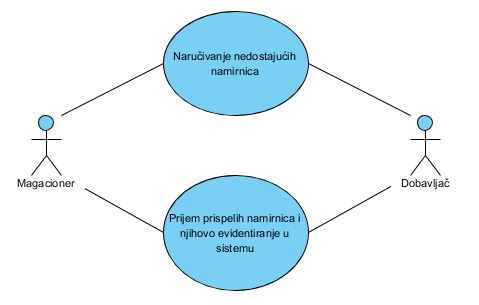
\includegraphics[width=136mm]{slike/Upravljanje_namirnicama.JPG}\\
% \begin{center}
% \caption{Slika 7. Dijagram slučajeva upotrebe}
% \end{center}
\begin{figure}[ht]
    \leavevmode
    \begin{center}
    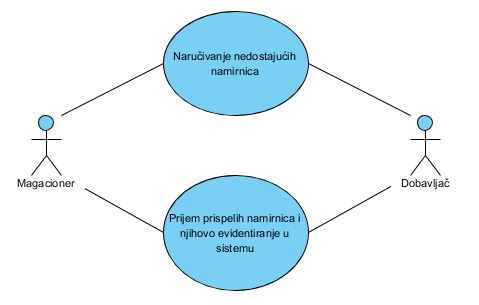
\includegraphics[height=0.5\textheight]{slike/Upravljanje_namirnicama.JPG}
    \end{center}
    \caption{Dijagram slu\v cajeva upotrebe} % opis ce stajati ispod slike
    \label{fig:slika5}
\end{figure}
 
 
 
 
 
 
 \subsubsection{Naručivanje nedostajućih namirnica}
 \begin{itemize}
    \item \textbf{Kratak opis}:
   Magacioner od dobavljača naručuje namirnice koje nedostaju u magacinu.
    \item \textbf{Učesnici}:
    Magacioner, dobavljač
    \item \textbf{Preduslovi}:
    U magacinu nedostaje izvesna količina određenih namirnica.
    \item \textbf{Postuslovi}:
    Dobavljaču je obavešten o količini i tipu namirnica koje treba da dobavi. 
    \item \textbf{Glavni tok}:
    \begin{enumerate}
        \item Magacioner pregledom inventara u sistemu utvrđuje da izvesna količina namirnica nedostaje.
        \item Magacioner pravi spisak koji sadrži sve namirnice koje će poručiti.
        \item Magacioner poziva dobavljača i poručuje namirnice sa spiska.
        \item Dobavljač saopštava magacioneru koje namirnice može u kom vremenskom roku da mu isporuči.
        \item Magacioner potvrđuje svoju porudžbinu.
    \end{enumerate}
\item \textbf{Alternativni tokovi}\\
        5.1. Magacioner otkazuje svoju porudžbinu. Slučaj upotrebe se nastavlja\\ na koraku 3 glavnog toka.
 
 \item \textbf{Dodatne informacije}
 \begin{itemize}
     \item 
    Magacioner otkazuje porudžbinu u slučaju da mu vremenski rok\\ koji mu dobavljač predlaže ne odgovara. Zatim poziva drugog dobavljača kako bi poručio namirnice.

 \end{itemize}
 \end{itemize}
 
  \subsubsection{Prijem prispelih namirnica i njihovo evidentiranje u sistemu}
 \begin{itemize}
    \item \textbf{Kratak opis}:
   Dobavljač isporučuje poručenu robu magacioneru. Magacioner smešta namirnice u magacin i evidentira nabavku u sistemu.
    \item \textbf{Učesnici}:
    Magacioner, dobavljač
    \item \textbf{Preduslovi}:
    Magacioner je poručio namirnice od dobavljača.
    \item \textbf{Postuslovi}:
    Magacin je dopunjen nedostajućim namirnicama i stanje magacina je ažurirano u sistemu. 
    \item \textbf{Glavni tok}:
    \begin{enumerate}
        \item Dobavljač pristiže na adresu restorana.
        \item Dobavljač obaveštava magacionera da je stigao.
        \item Dostavljač i magacioner se sastaju.
        \item Magacioner plaća dostavljaču.
        \item Dostavljač predaje robu magacioneru.
        \item Magacioner smešta robu u magacin.
        \item Magacioner u sistemu evidentira pristiglu nabavku.
        \item Sistem ažurira stanje namirnica u magacinu.  
        
    \end{enumerate}

\end{itemize}
 
 
